%%%%% vpc

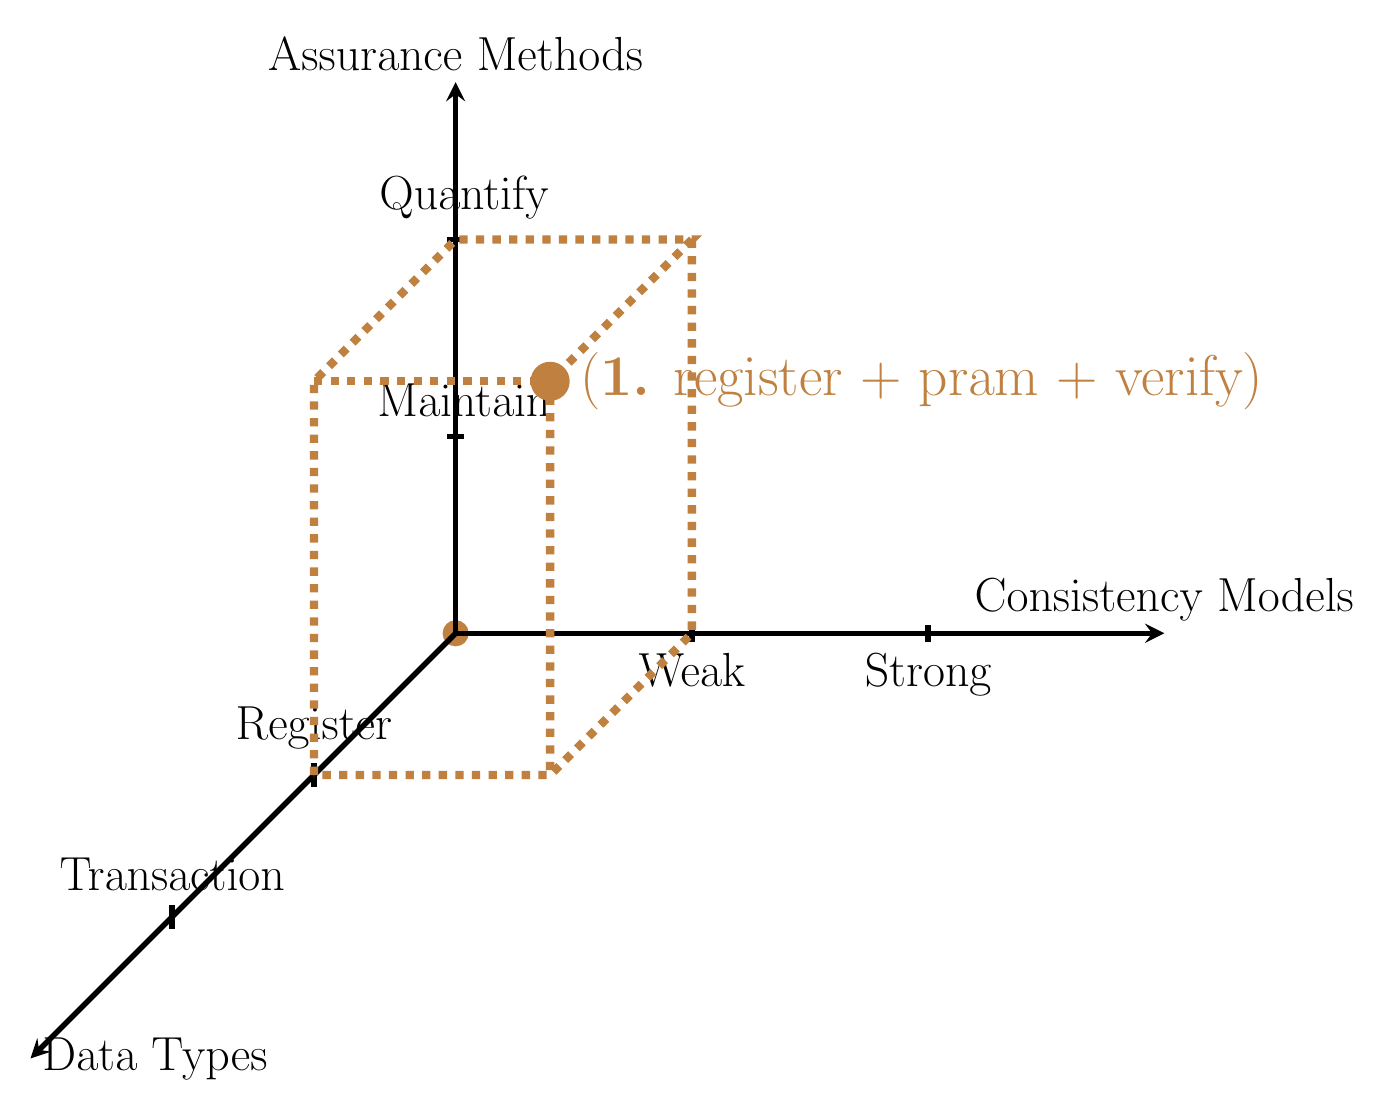
\begin{tikzpicture}[x = 0.5cm, y = 0.5cm, z = 0.3cm, >=stealth, font = \LARGE]

\begin{scope}[axesfont/.style = {font = \LARGE}, axesline/.style = {->, line width = 2}, 
  tickline/.style = {line width = 2}, tickfont/.style = {font = \LARGE}]

% the origin
\node[fill = brown, circle] at (0,0,0) {};
% The axes
\draw[axesline] (xyz cs:x=0) -- (xyz cs:x = 18) node[above, axesfont] {$\textrm{Consistency Models}$};
\draw[axesline] (xyz cs:y=0) -- (xyz cs:y = 14) node[above, axesfont] {$\textrm{Assurance Methods}$};
\draw[axesline] (xyz cs:z=0) -- (xyz cs:z = -18) node[right, axesfont] {$\textrm{Data Types}$};

% The ticks

% ticks for consistency models
\draw[tickline] (6,-3pt) -- (6,3pt) node[below = 6pt, tickfont] {Weak};
\draw[tickline] (12,-3pt) -- (12,3pt) node[below = 6pt, tickfont] {Strong};

% ticks for assurance methods
\draw[tickline] (-3pt,5) -- (3pt,5) node[above = 3pt, tickfont] {Maintain};
\draw[tickline] (-3pt,10) -- (3pt,10) node[above = 3pt, tickfont] {Quantify};

% ticks for data types
\draw[tickline] (xyz cs:y=-0.3pt,z=-6) -- (xyz cs:y=0.3pt,z=-6) node[above = 1pt, tickfont] {Register};
\draw[tickline] (xyz cs:y=-0.3pt,z=-12) -- (xyz cs:y=0.3pt,z=-12) node[above = 1pt, tickfont] {Transaction};
\end{scope}

%%%%%%%%%% for VPC: register + weak (pram) + quantify (verify)
  \begin{scope}[line/.style = {line width = 3, dashed, brown}]
	\draw[line]
	  (xyz cs:z = -6) coordinate (z) --
	  (xyz cs:y = 10, z = -6) coordinate (yz) --
	  (xyz cs:x = 0, y = 10, z = 0) coordinate (y) --
	  (xyz cs:x = 6, y = 10) coordinate (xy) --
	  (xyz cs:x = 6, y = 10, z = -6) coordinate (xyz) --
	  (xyz cs:x = 6, z = -6) coordinate (xz) -- cycle;
	\draw[line] (yz) -- (xyz);
	\draw[line] (xy) -- (6,0) -- (xz);
	
    % Dots and labels for P, Q
    \node[fill = brown, circle, inner sep = 5pt, label = {[brown, font = \huge] 0: (\textbf{1.}
  register + pram + verify)}] at (xyz) {};
  \end{scope}
\end{tikzpicture}
\end{document}
